\documentclass[xcolor=svgnames,17pt]{beamer}

\usepackage[export]{adjustbox}
\usepackage{bashful}
\usepackage{bookmark}
\usepackage{colortbl} \arrayrulecolor[gray]{0.7}
\usepackage{microtype}
\usepackage{pgfpages}
\usepackage{rotating}
\usepackage{textcomp}
\usepackage{tabularx}
\usepackage{xspace}
\usepackage{verbatim}

\usepackage{fontspec}

\hypersetup{pdfpagemode=,colorlinks=true,urlcolor=blue}

%\urlstyle{same}

\newcommand*{\sizefont}[1]{%
    \ifcase#1\relax
    \or \tiny
    \or \scriptsize
    \or \footnotesize
    \or \small
    \or \normalsize
    \or \large
    \or \Large
    \or \LARGE
    \or \huge
    \or \Huge
    \fi}

%%

\newcommand*{\mybullet}{\tikz[baseline=-.6ex]\node[%
    draw,circle,inner sep = -0.15ex,fill]{.};\xspace}

%\setbeamertemplate{footline}{
%    \usebeamercolor[fg]{page number in head/foot}%
%    \usebeamerfont{page number in head/foot}%
%    \hspace*{1ex}\insertframenumber\,/\,\inserttotalframenumber\hfill
%    github.com/andrewdotn/...\ }

\newcommand*{\plainfooter}{%
    \setbeamertemplate{footline}{
        \usebeamercolor[fg]{page number in head/foot}%
        \usebeamerfont{page number in head/foot}%
        \hspace*{1ex}\insertframenumber\,/\,\inserttotalframenumber\vskip2pt}}

\makeatletter
\def\alphslide{\@alph{\intcalcAdd{1}{\intcalcSub{\thepage}{\beamer@framestartpage}}}}
\newcommand*{\plainstepfooter}{
    \setbeamertemplate{footline}{
        \usebeamercolor[fg]{page number in head/foot}%
        \usebeamerfont{page number in head/foot}%
        \hspace*{1ex}\insertframenumber\alphslide\,/\,\inserttotalframenumber\vskip2pt}}
\makeatother

\setbeamertemplate{note page}{
    \sizefont{3}
    \setlength{\parskip}{10pt}
    \insertnote
    \par}

\setbeamertemplate{navigation symbols}{}
\setbeamerfont{title}{size=\LARGE}
\setbeamerfont{frametitle}{size=\LARGE}
\setbeamerfont{framesubtitle}{size=\normalsize}

\newcommand*{\tocsection}[1]{\pdfbookmark[2]{#1}{#1}}

\lstdefinestyle{bashfulStdout}{
    basicstyle=\ttfamily,
    keywords={},
    showstringspaces=false
}%

%%

\title{Adding third-party sign-on to a Django site}

\author{\texorpdfstring{%
    Andrew Neitsch}{Andrew Neitsch}}

\date{\small 2019-01-23}

\begin{document}

\tocsection{Title page}

\begin{frame}[plain]{\large\href{https://pyyyc.org/presentations/2019-01-23}{
    pyyyc.org/presentations/2019-01-23}}

\begin{tabular}{rl}
6:45ish & Talks \\
• & Adding third-party sign-on to django \\
\\[0.5ex]
\hline \\[-2ex]
& General Q\&A
\\[0.5ex]
\hline \\[-2ex]
& Socializing
\end{tabular}
\end{frame}

\begin{frame}[plain]{Thank you to our sponsor}

\includegraphics[center]{assembly.pdf}
\end{frame}

\begin{frame}[plain]{Thank you to our sponsor}

\includegraphics[center]{teamit-logo.png}
\end{frame}

\begin{frame}{polyglotyeg.com}

\includegraphics[width=0.7\paperwidth,center]{polyglot.pdf}
\end{frame}

%\sizefont{4}

\begin{frame}[plain]
\titlepage
\end{frame}

\begin{frame}{Outline}
\tableofcontents
\end{frame}

\section{Motivation}

\begin{frame}{Why use third-party sign-on?}
\begin{itemize}
\item Speed and convenience for users
\pause
\item Rich data and integrations with other sites
\only<2>{\\ Example: share with your friends}
\pause
\item Spam
\only<3>{\\ Malicious programs will sign up for your site to post spam}
\pause
\item Storing passwords is hard and makes you a hacking target
\end{itemize}
\end{frame}

\section{Walkthrough}

\begin{frame}
\tableofcontents[currentsection]
\end{frame}

\begin{frame}{Getting the code working}
\begin{enumerate}
\item Check out
\href{https://github.com/py-yyc/oauth_meetup}{github.com/py-yyc/oauth\_meetup}

\item Run \texttt{pipenv install}

\item \texttt{pipenv run ./manage.py migrate} \\
to create the database tables
\end{enumerate}
\end{frame}

\begin{frame}[plain]
4. Go to \url{https://secure.meetup.com/meetup_api/oauth_consumers/create}
\\ Enter anything for the consumer name,
\texttt{http://localhost:8000/oauth/login} for the ‘Redirect URI.’
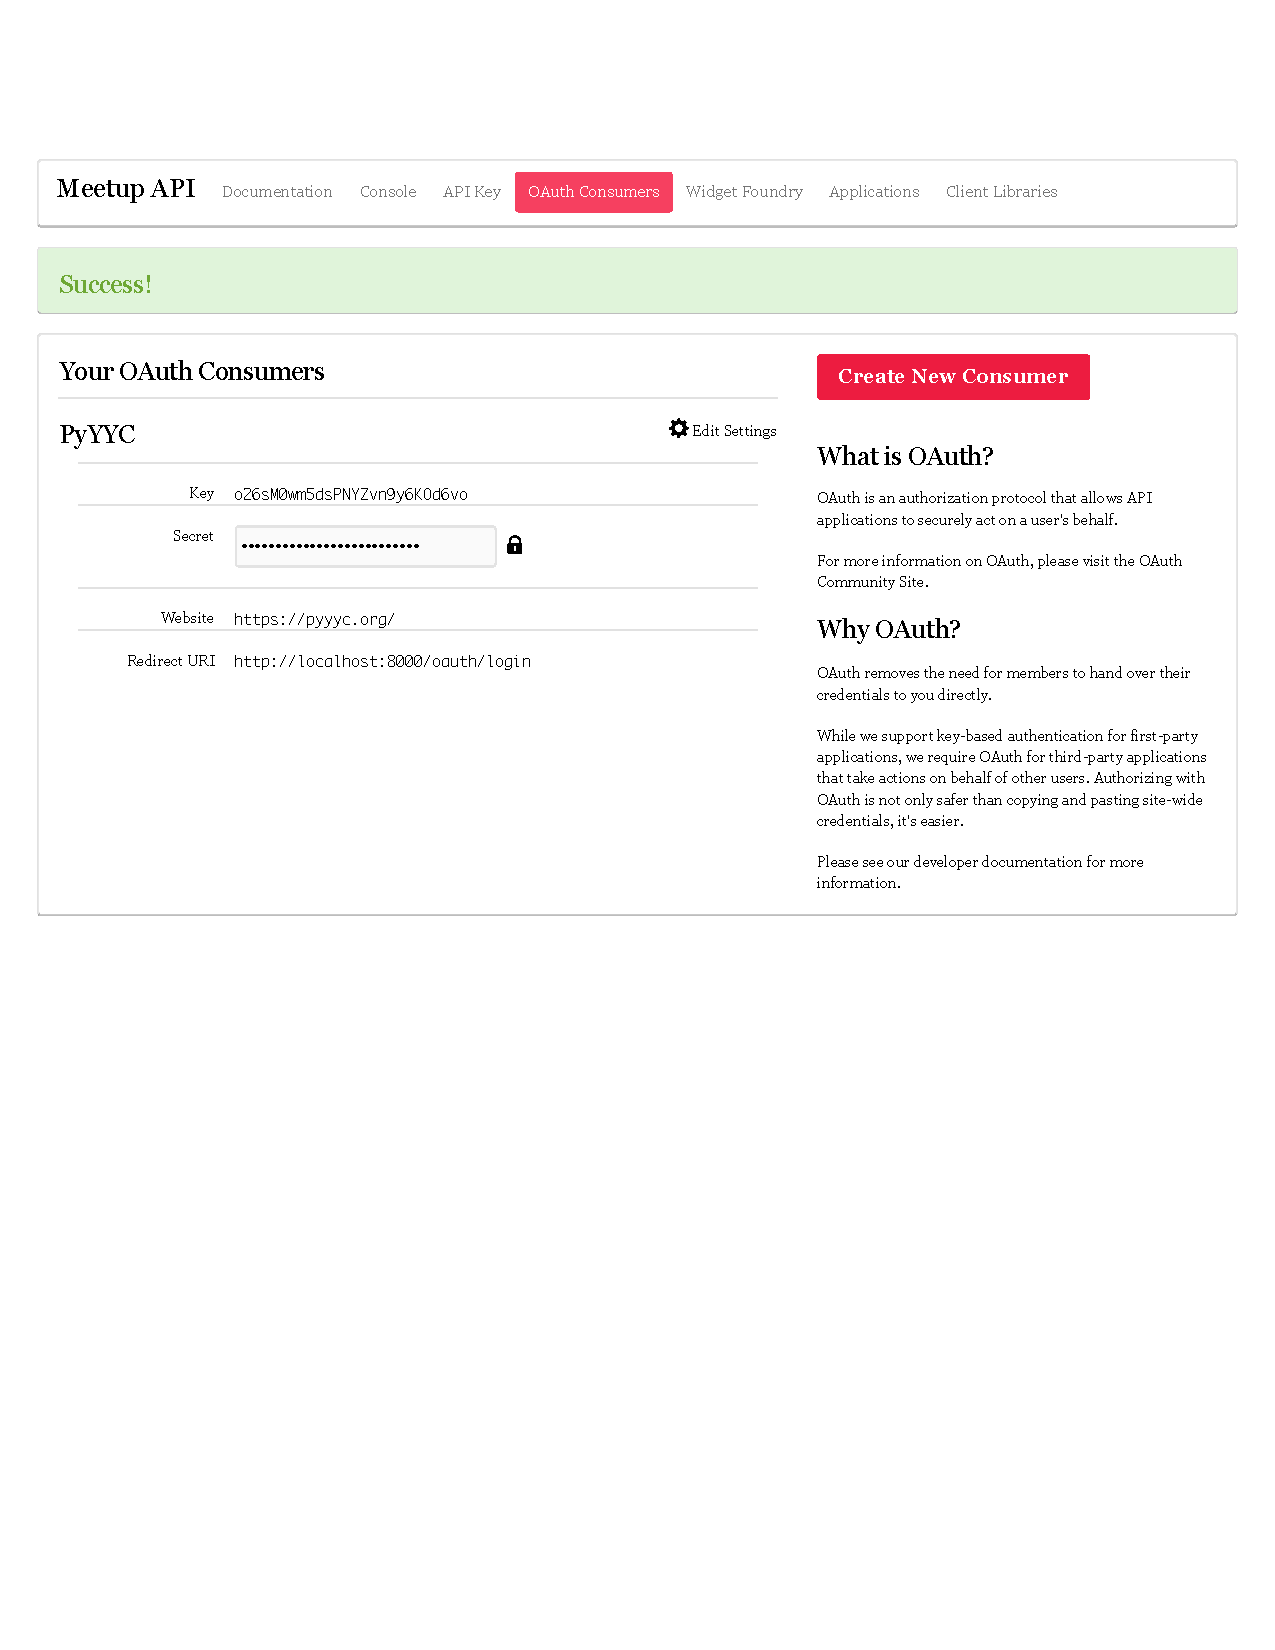
\includegraphics[width=0.5\paperwidth,center]{meetup-oauth-consumers.pdf}
\end{frame}

\begin{frame}[plain]
\begin{enumerate}
\setcounter{enumi}{4}
\item Add \texttt{MEETUP\_CLIENT\_ID} and \texttt{MEETUP\_CLIENT\_SECRET} to
\texttt{.django\_secrets.json}
\item \texttt{pipenv run ./manage.py runserver}
\end{enumerate}
\end{frame}

\begin{frame}[plain]
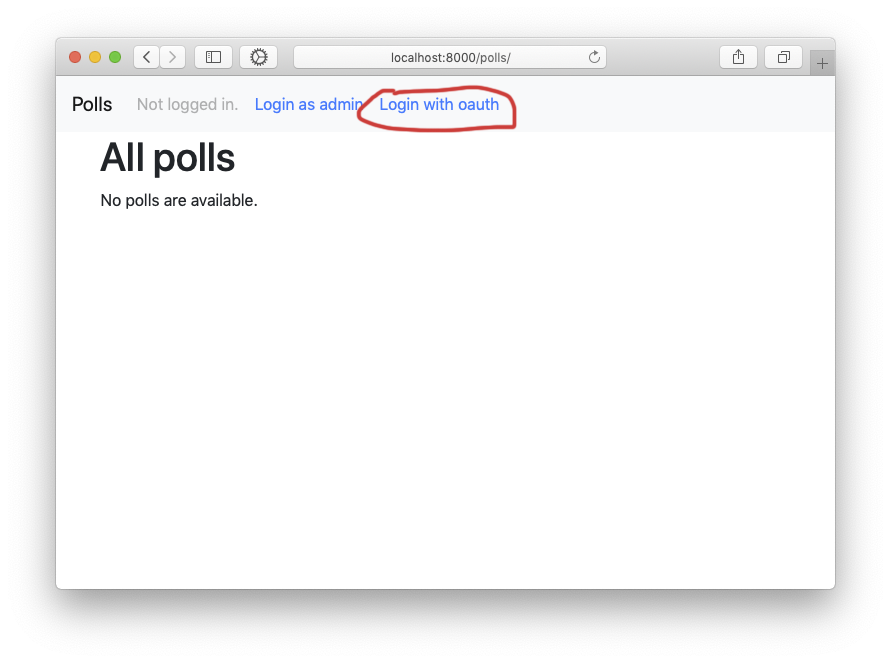
\includegraphics[width=0.9\paperwidth,center]{flow1.png}
\end{frame}

\begin{frame}[plain]
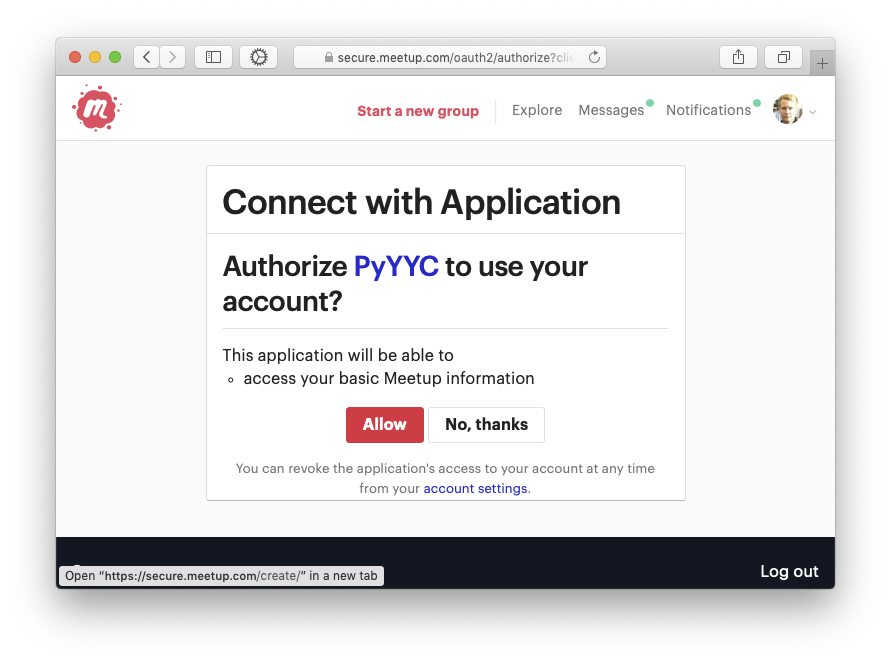
\includegraphics[width=0.9\paperwidth,center]{flow2.png}
\end{frame}

\begin{frame}[plain]
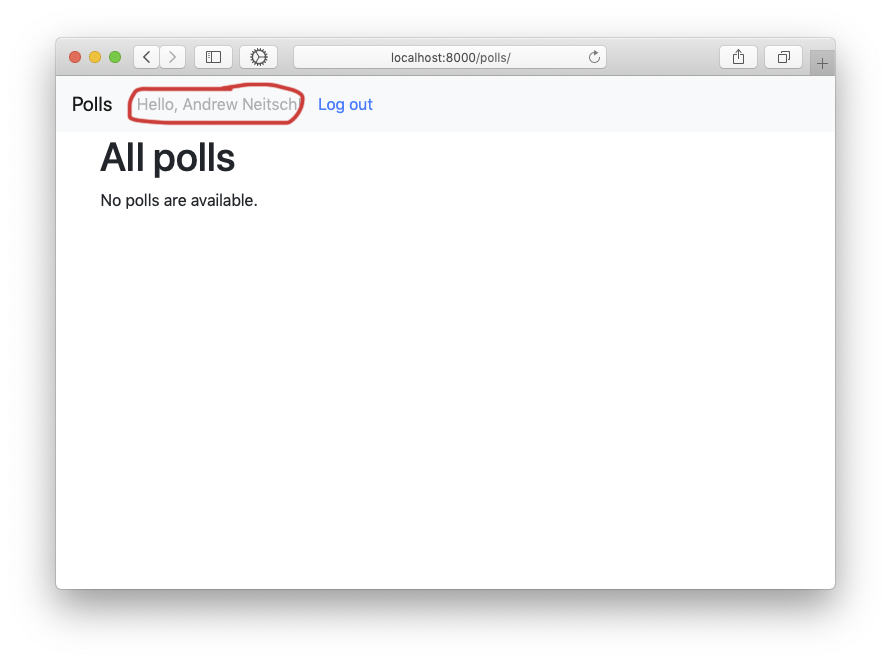
\includegraphics[width=0.9\paperwidth,center]{flow3.png}
\end{frame}

\begin{frame}[fragile]
\sizefont{2}
\begin{verbatim}
Starting development server at http://127.0.0.1:8000/
Quit the server with CONTROL-C.
{'country': 'ca', 'city': 'Calgary', 'topics': [{'urlkey':
'opensource', 'name': 'Open Source', 'id': 563}, {'urlkey':
'computer-programming', 'name': 'Computer programming', 'id':
48471}, {'urlkey': 'programming-languages', 'name':
'Programming Languages', 'id': 17628}, {'urlkey': 'webdesign',
'name': 'Web Design', 'id': 659}, {'urlkey': 'ixd', 'name':
'Interaction Design', 'id': 10110}], 'joined': 1009868400000,
'link': 'http://www.meetup.com/members/2390428304', 'photo':
{'highres_link': 'https://secure.meetupstatic.com/photos/member/e/7/2/4/
'lon': -114.08000183105469, 'other_services': {},
'name': 'Andrew Neitsch', 'visited': 1548129478000, 'self':
{'common': {}}, 'id': 2390428304, 'state': 'AB', 'lang': 'en_US',
'lat': 51.04999923706055, 'status': 'active'}
\end{verbatim}
\end{frame}

\section{How OAuth works}

\begin{frame}
\tableofcontents[currentsection]
\end{frame}

\begin{frame}[plain]
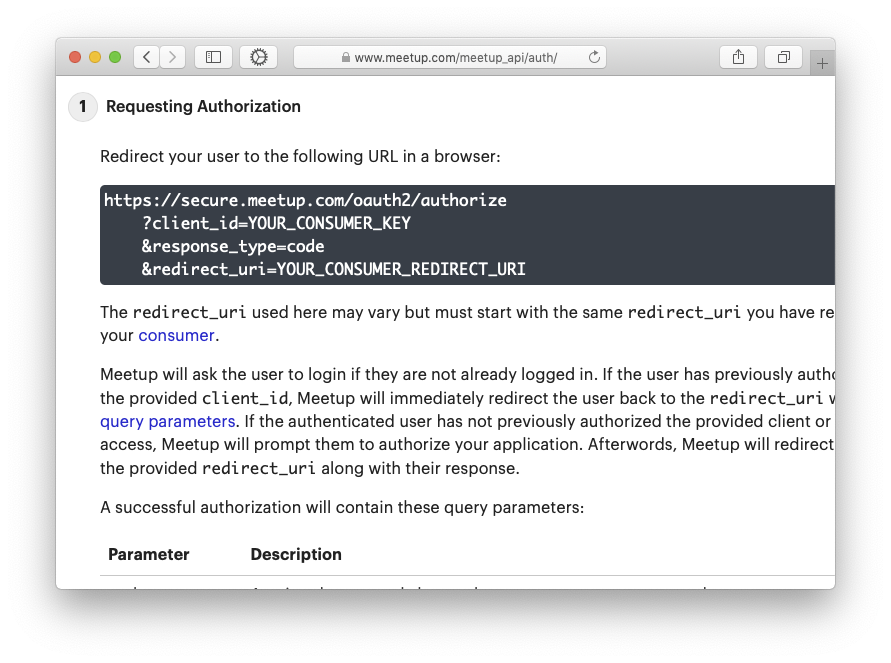
\includegraphics[width=0.9\paperwidth,center]{how-oauth-works.png}
\end{frame}

\begin{frame}[plain]
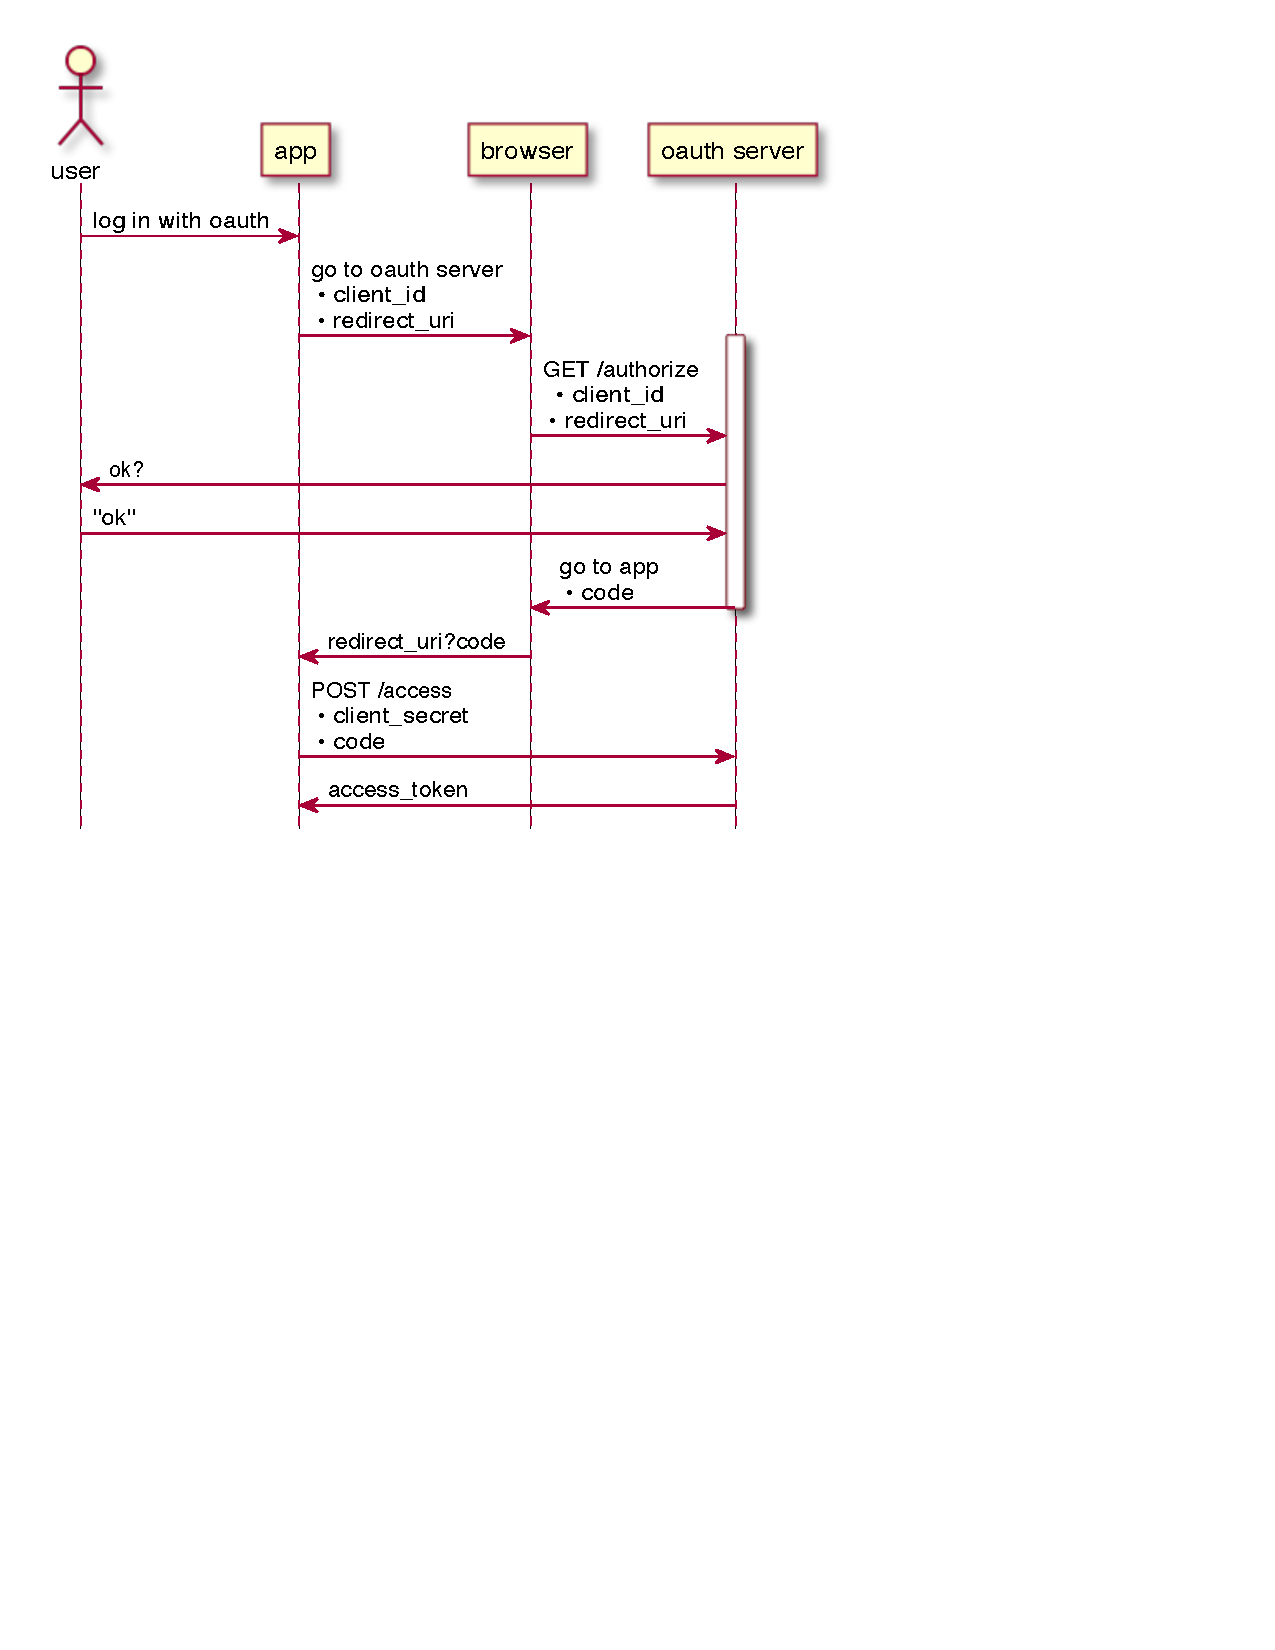
\includegraphics[width=0.7\paperwidth,center]{uml-flow1.pdf}
\end{frame}

\begin{frame}{Security properties}
\begin{itemize}
\item User only clicks ok on a trusted site
\item The app is protected from impersonation by the server checking
\texttt{redirect\_uri}
\item The app proves its identity with \texttt{client\_secret}, which is
never disclosed to the user or browser
\item The app POSTs to a trusted server to get an access token
\end{itemize}
\end{frame}

\begin{frame}{After initial login}
The access token is meant for the app to impersonate the user!

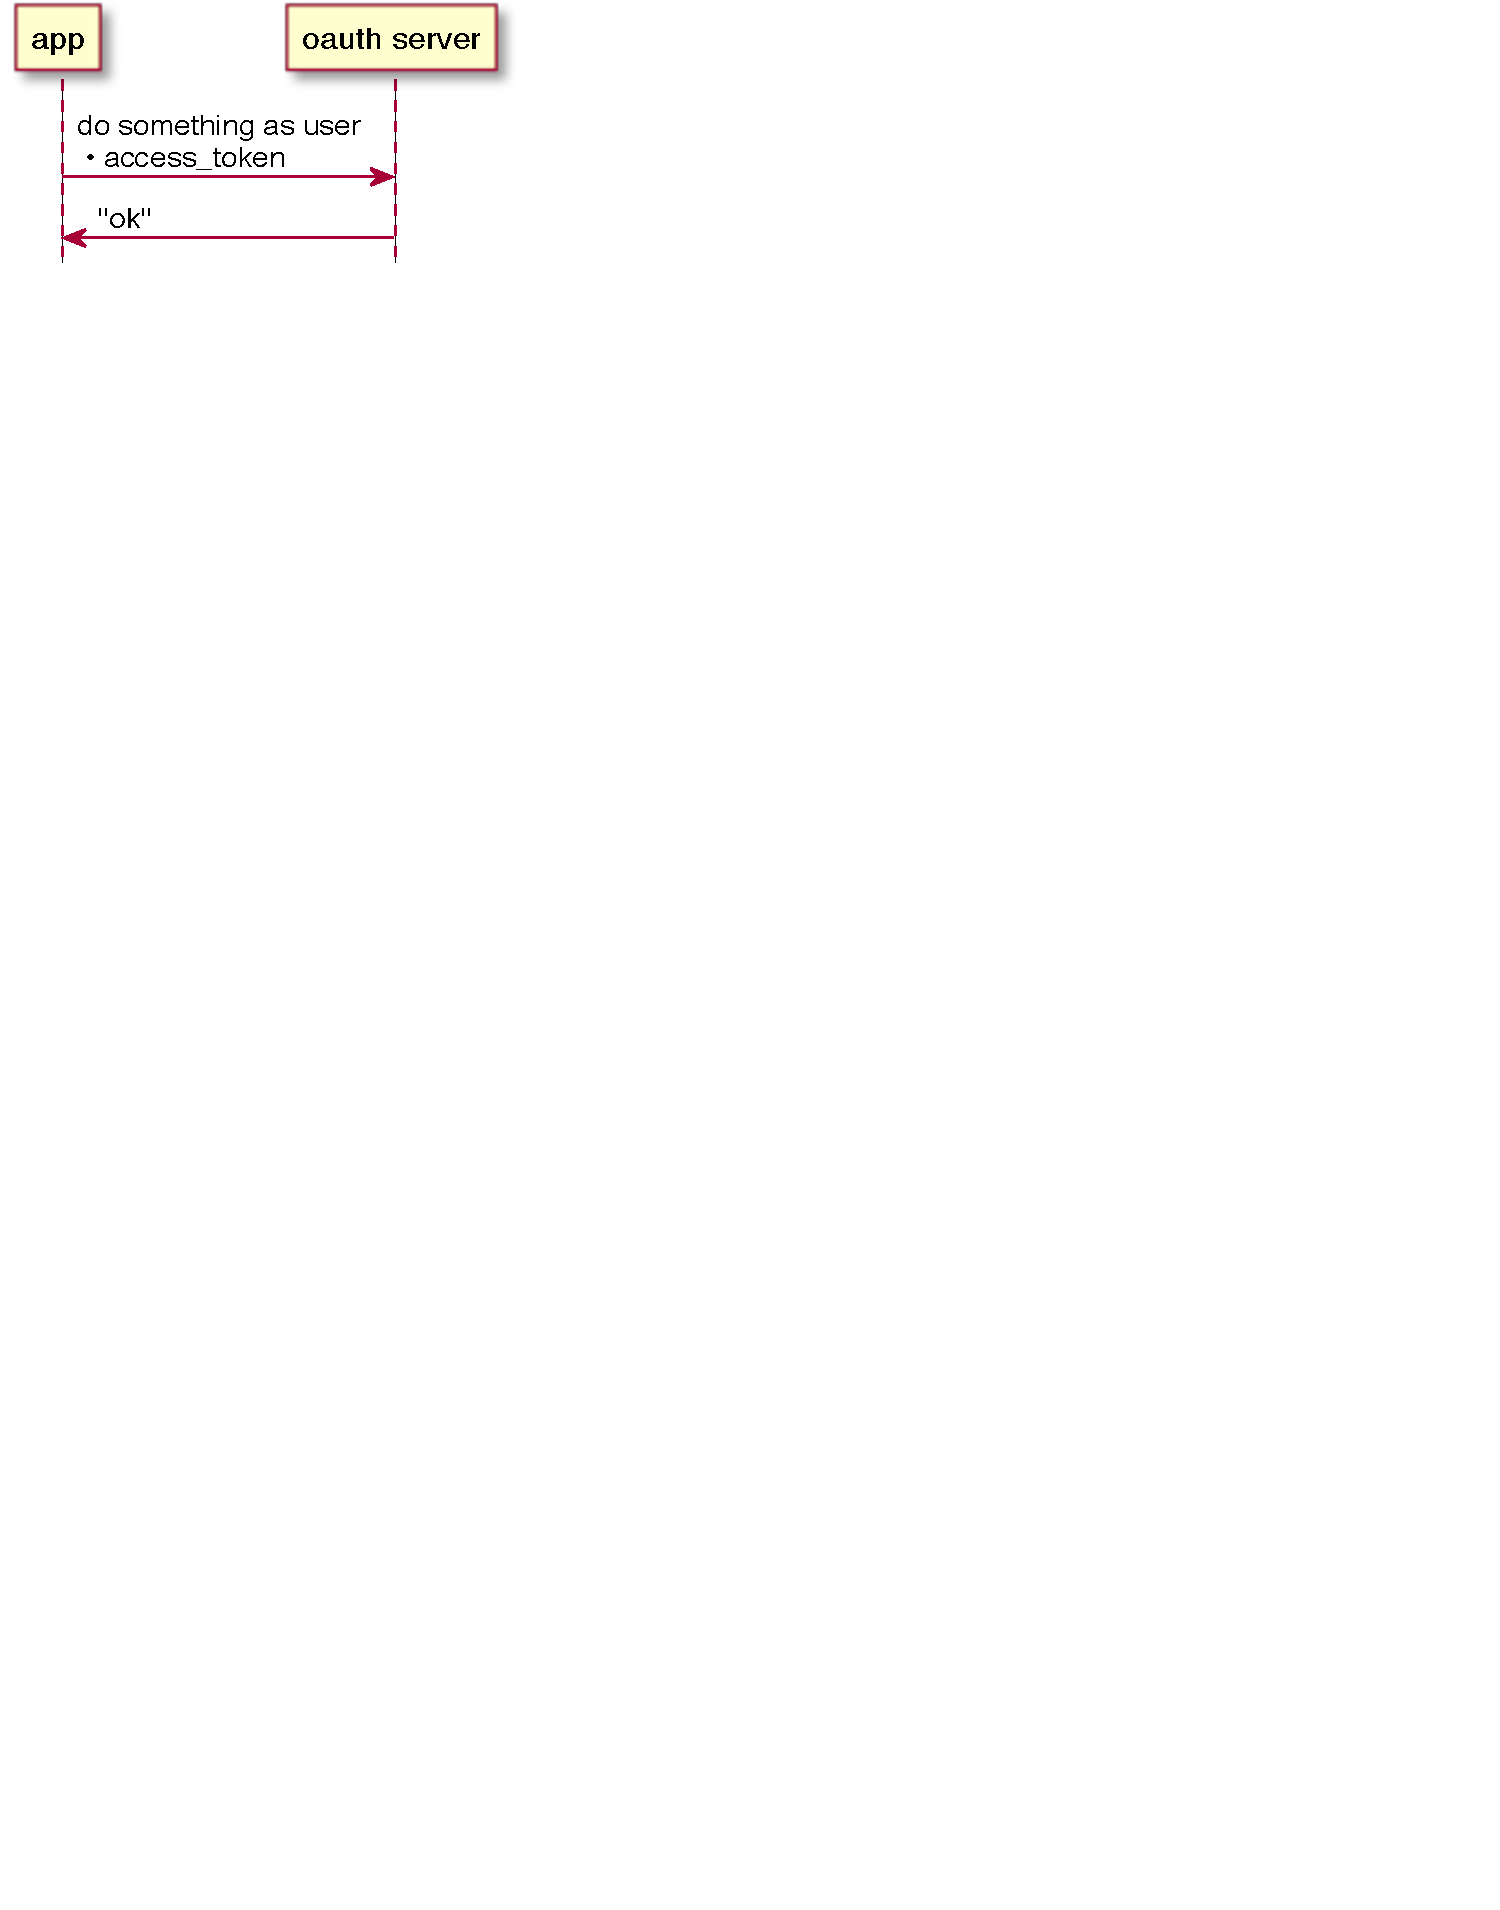
\includegraphics[width=0.6\paperwidth,center]{uml-flow2.pdf}

Note that the user and browser are now out of the picture.
\end{frame}

\begin{frame}{The Meetup API is powerful}
\begin{itemize}
\item Personal interests
\item Photos of you
\item Your location history
\item Private messages
\end{itemize}

Mixing authentication and authorization.
\end{frame}

\begin{frame}{Beware}
\begin{itemize}
\item Third-party sign-on is convenient
\pause
\item But the convenient data sharing goes both ways
\pause
\item The site using third-party sign-on learns a lot about you
\pause
\item And the site offering third-party sign-on learns about where you go
on the internet and what you do there
\end{itemize}
\pause
When developing apps: don’t be evil!
\end{frame}

\section{The code}

\begin{frame}{The code}
\begin{itemize}
\item \texttt{tests.py}
\only<1>{Uses \texttt{responses}, fake OAuth server}
\pause
\item \texttt{views.py}
\only<2>{if code, post to \texttt{/access}, then get \texttt{/member/self}}
\\ Get or create a User object identified by meetup user ID
\\ \texttt{login(request, user)}
\item \texttt{base.html}
\end{itemize}
\only<3>{Only about 50 lines of code in \texttt{views.py}! \\ no error
handling though}
\end{frame}

\section{Conclusion}

\begin{frame}
\tableofcontents[currentsection]
\end{frame}

\begin{frame}{Possible enhancements}
\begin{itemize}
\item Use a library like
\url{https://docs.authlib.org/en/latest/client/django.html}
\item Maintain access by refreshing tokens on a timer
\item Store a reasonable subset of user data in the DB
\item Send \texttt{state} in initial \texttt{/authorize} call*
\end{itemize}
\end{frame}

\begin{frame}{Conclusion}
\begin{itemize}
\item Pretty straightforward
\end{itemize}
\end{frame}

\end{document}
